% !TEX root = ../report.tex

\chapter{Аналитическая часть}

В данном разделе проводится анализ предметной области онлайн-маркетплейсов, включающий:

\begin{itemize}
    \item определение понятия онлайн-маркетплейса и его отличий от классического интернет-магазина;
    \item оценку существующих решений на рынке электронной коммерции;
    \item формализацию задач, решаемых проектируемой системой;
    \item описание ролей пользователей приложения;
    \item описание структур данных, необходимых для хранения информации о товарах, заказах, пользователях и связанных сущностях.
\end{itemize}

На основе проведённого анализа формируются следующие результаты:
\begin{itemize}
    \item перечень ролей пользователей проектируемой системы;
    \item определение сценариев использования системы для каждой роли;
    \item создание диаграмм: \begin{itemize}
        \item вариантов использования;
        \item сущность-связь в нотации Чена.
    \end{itemize}
    \item выбор модели БД, достаточной для решения поставленной задачи.
\end{itemize}

% !TEX root = ../../report.tex

\section{Анализ предметной области}

\textbf{Онлайн-маркетплейс} --- электронная торговая площадка, на которой множество независимых продавцов размещают свои товары, а покупатели выбирают и заказывают их через единый интерфейс~\cite{marketplace_def}. В отличие от классического интернет-магазина, маркетплейс не владеет товарами и не осуществляет их закупку: платформа выступает посредником между продавцом и покупателем, предоставляя инфраструктуру для размещения каталога, приёма заказов и сбора обратной связи.

По данным Ассоциации компаний интернет-торговли (АКИТ), объём интернет-торговли в России по итогам 2025 года составил 11,5~трлн рублей, что соответствует росту на 28\% относительно предыдущего года~\cite{akit2025}. Доля онлайн-продаж достигла 18,8\% от всего розничного товарооборота. Маркетплейсы являются значимой частью рынка онлайн-торговли.

Ключевые бизнес-процессы маркетплейса включают:

\begin{itemize}
    \item регистрацию продавцов и размещение товаров с привязкой к категориям;
    \item просмотр каталога покупателями с возможностью фильтрации и поиска;
    \item оформление заказов с фиксацией цены на момент покупки;
    \item управление жизненным циклом заказа (от корзины до доставки);
    \item систему отзывов и рейтингов, обеспечивающую обратную связь;
    \item формирование аналитической отчётности для продавцов и аналитиков.
\end{itemize}

Рассмотренные далее маркетплейсы являются закрытыми коммерческими системами. В проектируемой системе отдельно рассматриваются каталог, заказы, отзывы, история изменения цен и отчётность продавца.


% !TEX root = ../../report.tex

\section{Анализ существующих решений}

Для определения функциональных требований к проектируемой системе проведён сравнительный анализ трёх распространённых маркетплейсов, доступных российским пользователям.

\begin{itemize}
    \item \textbf{Ozon} --- маркетплейс с интерфейсом для продавцов, покрывающим управление товарами, заказами, аналитикой и финансами. Предоставляет расширенную аналитику в личном кабинете продавца, часть функций доступна по подписке. Поддерживает раздельные рейтинги товара и продавца~\cite{ozon};
    \item \textbf{Wildberries} --- маркетплейс с личным кабинетом продавца, охватывающим товары, заказы, поставки и продвижение. Базовая аналитика встроена в платформу бесплатно; для расширенной требуются сторонние сервисы. Поддерживаются раздельные рейтинги товара и продавца~\cite{wildberries};
    \item \textbf{AliExpress} --- трансграничная торговая площадка, ориентированная на международных продавцов. Базовая аналитика доступна в кабинете продавца. Поддерживаются рейтинги товара и продавца~\cite{aliexpress}.
\end{itemize}

Критерии сравнения соответствуют характеристикам, которые используются в проектируемой системе:

\begin{enumerate}
    \item открытость модели данных;
    \item история изменения цен товара;
    \item бесплатная встроенная аналитика продаж;
    \item раздельные рейтинги товара и продавца;
    \item выделенная роль аналитика только для чтения;
    \item логистика как часть предметной области.
\end{enumerate}

Сравнение платформ по сформированным критериям приведено в таблице~\ref{tbl:comparison}.

\begin{table}[h!]
    \caption{Сравнение существующих решений}
    \label{tbl:comparison}
    \centering
    \small
    \begin{tabular}{|l|l|l|l|l|}
        \hline
        \textbf{Критерий} & \textbf{Ozon} & \textbf{Wildberries} & \textbf{AliExpress} & \makecell[l]{\textbf{Проектируемая}\\\textbf{система}} \\ \hline
        \makecell[l]{Открытость\\модели данных} & Нет & Нет & Нет & Да \\ \hline
        \makecell[l]{История\\цен товара} & \makecell[l]{Не\\раскрывается} & \makecell[l]{Не\\раскрывается} & \makecell[l]{Не\\раскрывается} & Да \\ \hline
        \makecell[l]{Бесплатная встроенная\\аналитика продаж} & Частично & Да & Да & Да \\ \hline
        \makecell[l]{Рейтинг товара\\и продавца} & Да & Да & Да & Да \\ \hline
        \makecell[l]{Выделенная роль\\аналитика\\только для чтения} & \makecell[l]{Не\\указана} & \makecell[l]{Не\\указана} & \makecell[l]{Не\\указана} & Да \\ \hline
        \makecell[l]{Логистика\\в предметной\\области} & Да & Да & Да & Нет \\ \hline
    \end{tabular}
\end{table}

Рассмотренные платформы являются закрытыми коммерческими системами.

В проектируемой системе выделяются открытая модель данных, хранение истории изменения цен и отдельная роль аналитика. Задача логистики не рассматривается.


% !TEX root = ../../report.tex

\section{Формализация задачи}

Необходимо спроектировать базу данных для онлайн-маркетплейса, обеспечивающую хранение и обработку данных о товарах, продавцах, покупателях, заказах, отзывах, категориях и адресах доставки.

Требуется разработать систему, предоставляющую пользователям интерфейсы взаимодействия с данными маркетплейса. В рамках системы должны быть предусмотрены следующие роли: гость, покупатель, продавец, администратор и аналитик.

Для указанных ролей необходимо определить сценарии взаимодействия с системой: просмотр каталога, управление товарами, оформление заказов, оставление отзывов, администрирование и формирование аналитической отчётности.

Проектируемая система ограничивается каталогом товаров, заказами, адресами доставки, отзывами и состояниями исполнения заказа. Задача логистики не рассматривается: в предметную область не включаются логистические компании, маршруты, курьеры, графики складов и события фактической передачи товара. Состояние исполнения заказа фиксируется статусами заказа.

\pagebreak


% !TEX root = ../../report.tex

\section{Описание ролей}

Исходя из анализа предметной области и требований к системе, выделены следующие роли пользователей:

\begin{enumerate}
    \item гость (неавторизованный пользователь);
    \item покупатель;
    \item продавец;
    \item администратор;
    \item аналитик.
\end{enumerate}

\textbf{Гость} --- неавторизованный пользователь, обладающий правами на просмотр каталога товаров, карточки товара (включая информацию о товаре, историю изменения цены и отзывы), а также на прохождение процедуры авторизации (регистрации или входа в систему).

\textbf{Покупатель} --- авторизованный пользователь, который, помимо возможностей гостя, может оформлять заказы (добавлять товары в корзину, выбирать адрес доставки, производить оплату) и оставлять отзывы на приобретённые товары. Каждый покупатель управляет собственными адресами доставки. Один покупатель может оставить не более одного отзыва на конкретный товар.

\textbf{Продавец} --- авторизованный пользователь, зарегистрировавший профиль компании. Продавец управляет собственными товарами (добавление, редактирование, удаление), просматривает входящие заказы и фиксирует их переходы по статусам отгрузки и доставки. Также продавцу доступна статистика продаж за указанный период.

\textbf{Администратор} --- пользователь с функциями модератора платформы. Наследует возможности гостя (просмотр каталога, карточки товара, авторизация). Администратор управляет категориями товаров (создание, редактирование, удаление), может удалять пользователей, продавцов, товары и отзывы. Также ему доступен просмотр всех заказов в системе, отчётов и статистики продаж. Администратор не создаёт товары, не оформляет заказы и не оставляет отзывы.

\textbf{Аналитик} --- пользователь, обладающий правами на чтение всех данных системы без возможности их модификации. Роль предназначена для формирования отчётов: топ товаров по продажам, динамика заказов по времени, распределение продаж по категориям.

Отдельная роль для управления складскими остатками не выделяется. Количество товара относится к данным товара, которыми управляет продавец, а резерв изменяется при обработке заказов.

Диаграмма вариантов использования приведена на рисунке~\ref{fig:usecase}.

\begin{figure}[H]
    \centering
    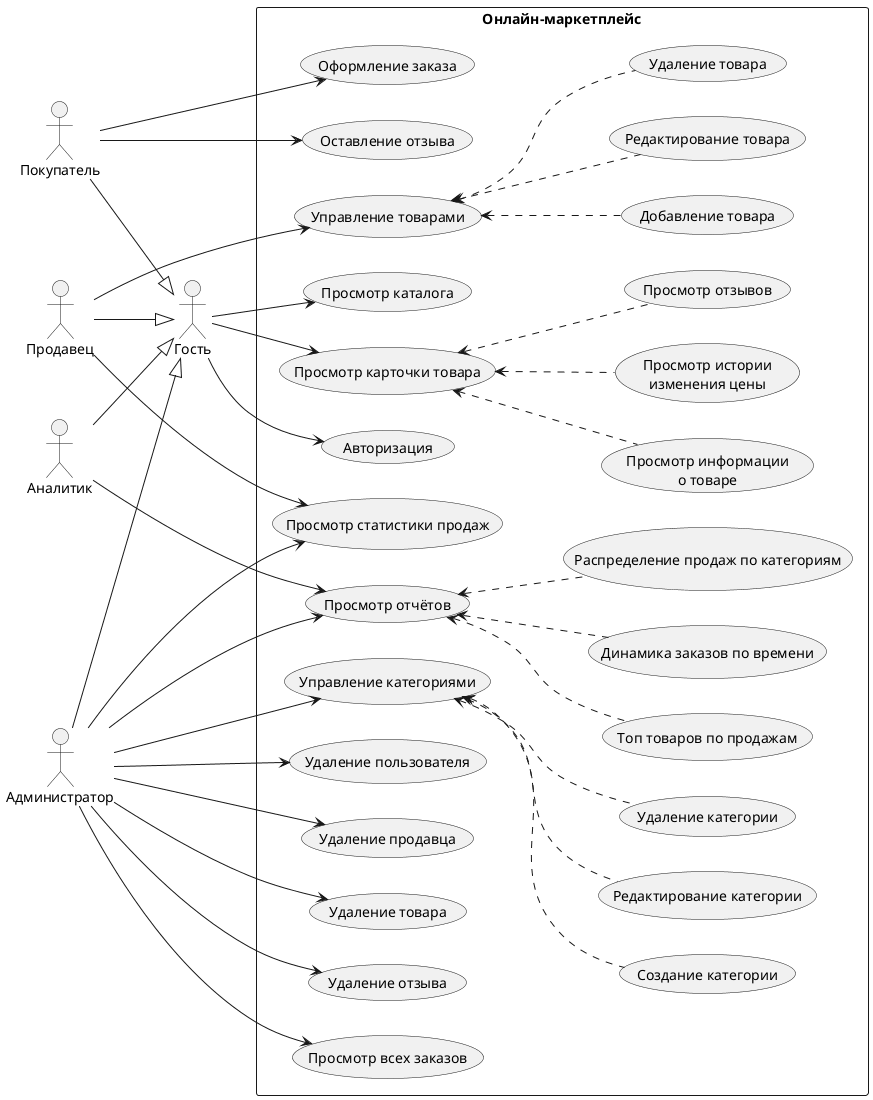
\includegraphics[width=\textwidth]{img/UseCases.png}
    \caption{Диаграмма вариантов использования}
    \label{fig:usecase}
\end{figure}

Каждая авторизованная роль наследует возможности гостя. Администратор, в отличие от покупателя и продавца, не наследует их бизнес-действий, а обладает собственным набором операций, ориентированных на модерацию и контроль данных платформы.


% !TEX root = ../../report.tex

\section{Описание данных и структур}

На основе анализа предметной области и сформулированных требований выделены следующие сущности:

\begin{itemize}
    \item пользователь;
    \item продавец;
    \item товар;
    \item категория;
    \item заказ;
    \item позиция заказа;
    \item отзыв;
    \item адрес доставки;
    \item история изменения цен.
\end{itemize}

Дополнительно выделена связующая сущность <<товар--категория>> для представления связи <<многие ко многим>> между товарами и категориями. Таким образом, общее число сущностей составляет 10.

Сведения о признаках сущностей приведены в таблице~\ref{tbl:entities}.

\begin{table}[H]
    \caption{Сведения о сущностях предметной области}
    \label{tbl:entities}
    \begin{tabular}{|l|l|}
        \hline
        \textbf{Сущность} & \textbf{Данные} \\ \hline
        Пользователь & \makecell[l]{Идентификатор, Email,\\ Данные авторизации, Полное имя,\\ Телефон, Роль} \\ \hline
        Продавец & \makecell[l]{Идентификатор, Пользователь,\\ Название компании, Описание, Рейтинг} \\ \hline
        Товар & \makecell[l]{Идентификатор, Продавец, Название,\\ Описание, Цена, Количество на складе,\\ Количество в резерве, Рейтинг} \\ \hline
        Категория & \makecell[l]{Идентификатор, Родительская категория,\\ Название, Описание} \\ \hline
        Заказ & \makecell[l]{Идентификатор, Покупатель,\\ Продавец для оформленного заказа,\\ Адрес доставки для оформленного заказа,\\ Статус, Итоговая сумма} \\ \hline
        Позиция заказа & \makecell[l]{Идентификатор, Заказ, Товар,\\ Количество, Цена на момент покупки} \\ \hline
        Отзыв & \makecell[l]{Идентификатор, Пользователь, Товар,\\ Оценка (1--5), Комментарий} \\ \hline
        Адрес доставки & \makecell[l]{Идентификатор, Пользователь, Город,\\ Улица, Дом, Квартира, Индекс,\\ Признак основного} \\ \hline
        История цен & \makecell[l]{Идентификатор, Товар, Старая цена,\\ Новая цена, Дата изменения, Кто изменил} \\ \hline
    \end{tabular}
\end{table}

Между сущностями установлены следующие связи:

\begin{itemize}
    \item пользователь~--- продавец: один к нулю или одному (профиль продавца связывается только с учётной записью, имеющей роль продавца);
    \item пользователь~--- заказ: один ко многим (покупатель оформляет несколько заказов);
    \item пользователь~--- адрес: один ко многим;
    \item пользователь~--- отзыв: один ко многим;
    \item продавец~--- товар: один ко многим;
    \item продавец~--- оформленный заказ: один ко многим;
    \item товар~--- категория: многие ко многим (через связующую сущность);
    \item товар~--- отзыв: один ко многим;
    \item товар~--- история цен: один ко многим;
    \item категория~--- категория: один ко многим (иерархия через ссылку на родительскую категорию);
    \item заказ~--- позиция заказа: один ко многим;
    \item оформленный заказ~--- адрес: многие к одному;
    \item позиция заказа~--- товар: многие к одному.
\end{itemize}

На рисунке~\ref{fig:ER} приведена концептуальная диаграмма сущность-связь в нотации Чена.

\begin{figure}[H]
    \centering
    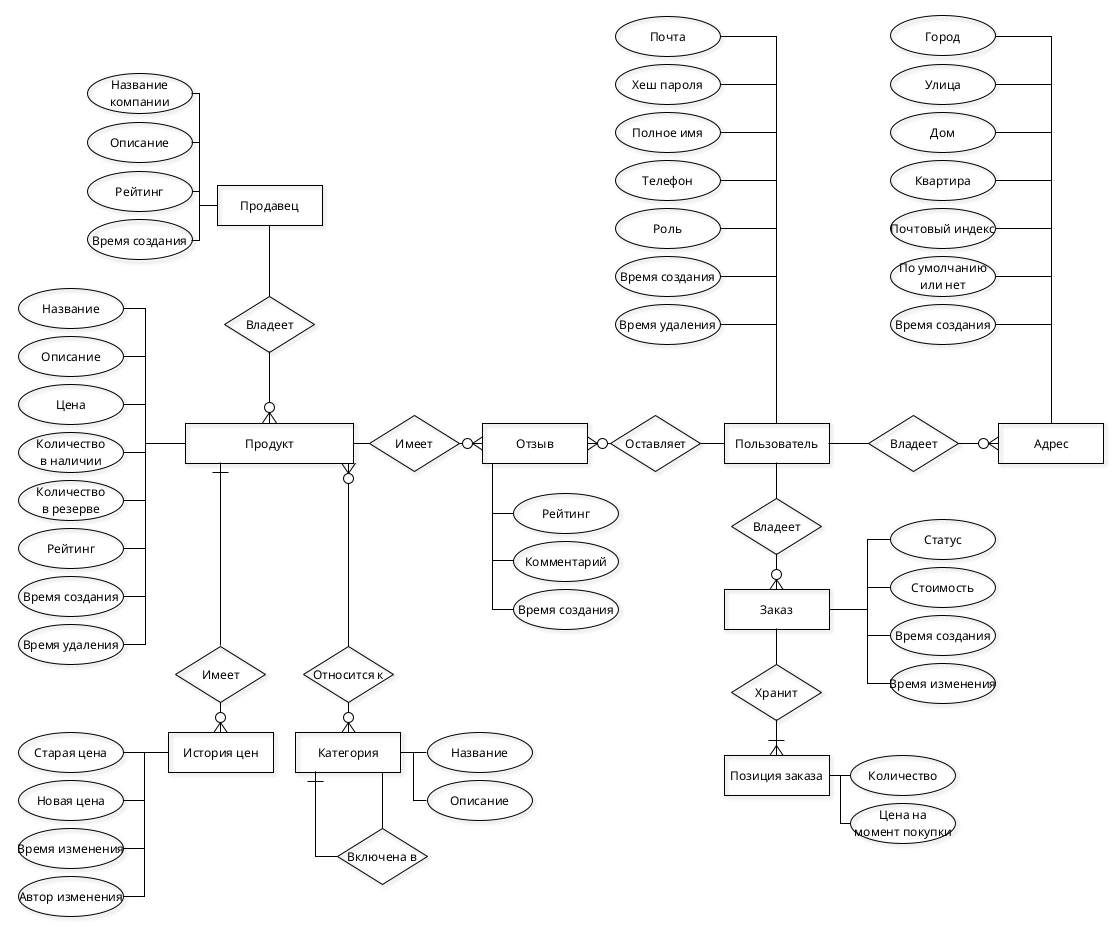
\includegraphics[width=\textwidth]{img/ER_Chen.png}
    \caption{Диаграмма сущность-связь в нотации Чена}
    \label{fig:ER}
\end{figure}

Бизнес-правило <<корзина как черновик заказа>> позволяет не выделять корзину в самостоятельную сущность. Черновик заказа не связан с адресом доставки и продавцом, а при оформлении разделяется на несколько заказов --- по одному на каждого продавца. В момент оформления фиксируется цена товара для соответствующей позиции заказа.

Для контроля доступного остатка товара учитываются общий остаток у продавца и количество товара, находящееся в резерве по оформленным заказам. Доступное для нового заказа количество определяется как разность общего остатка и зарезервированного количества.

Жизненный цикл заказа включает состояния черновика, ожидания оплаты, оплаты, отгрузки, доставки и отмены. При оформлении заказа товар резервируется. При отмене заказа или истечении срока оплаты резерв освобождается. При отгрузке уменьшается общий складской остаток и соответствующее количество в резерве. Отмена заказа допускается до отгрузки.

Для формирования аналитической отчётности необходимы показатели по продавцу за временной интервал: количество заказов, общая выручка, средний чек и наименование самого продаваемого товара.


% !TEX root = ../../report.tex

\section{Анализ моделей баз данных}

Для выбора модели хранения данных рассмотрены три группы моделей: дореляционные, реляционные и постреляционные~\cite{db_models}. Сравнение выполняется по признакам, связанным с проектируемой системой: фиксированность схемы, наличие стандартного языка запросов, возможность хранения неструктурированных данных и поддержка целостности.

Дореляционные модели используют иерархические или сетевые связи между записями с жёстко заданной схемой и структурированными записями. Такая организация усложняет изменение связей и выполнение декларативных запросов к данным~\cite{db_models}. Постреляционные модели расширяют реляционный подход средствами хранения составных и полуструктурированных данных. Для текущей задачи такие возможности не являются основными, так как каталог, заказы, пользователи и отзывы имеют заранее определённые атрибуты и связи.

Реляционная модель представляет данные в виде отношений, поддерживает ключи, внешние связи и стандартный язык запросов~\cite{db_models, relation_model}. Эти свойства соответствуют требованиям проектируемой системы: требуется хранить связанные сущности, контролировать целостность данных и разграничивать доступ к ним.

Сравнение рассмотренных групп моделей представлено в таблице~\ref{tbl:model_comparison}.

\begin{table}[H]
    \caption{Сравнение моделей БД}
    \label{tbl:model_comparison}
    \centering
    \begin{tabular}{|l|l|l|l|}
        \hline
        \multicolumn{1}{|c|}{\multirow{2}{*}{\textbf{Критерий}}} & \multicolumn{3}{c|}{\textbf{Модель}} \\ \cline{2-4}
        \multicolumn{1}{|c|}{} & \makecell[l]{Дореля-\\ционная} & \makecell[l]{Реля-\\ционная} & \makecell[l]{Постреля-\\ционная} \\ \hline
        \makecell[l]{Фиксированная\\схема данных} & Да & Да & Частично \\ \hline
        \makecell[l]{Стандартный\\язык запросов} & Нет & Да & Да \\ \hline
        \makecell[l]{Хранение неструкту-\\рированных данных} & Нет & Нет & Да \\ \hline
        \makecell[l]{Обеспечение\\целостности данных} & Частично & Да & Частично \\ \hline
    \end{tabular}
\end{table}

Для проектируемой системы выбрана \textbf{реляционная модель} базы данных. Она соответствует структуре данных онлайн-маркетплейса и позволяет описать связи между товарами, заказами, пользователями, отзывами и категориями средствами ограничений целостности.

